\documentclass{article}

\usepackage{graphicx}


\begin{document}

\section{Agenda}
\begin{itemize}
	\item Current Situation    (25 min)
        \item Envisioned future    (25 min)
        \item Company Structure    (10 min)
        \item Convincing Total     (25 min)	
        \item IP concerns          (25 min)
        \item Milestones           (15 min)
\end{itemize}

\section{Current Situation}


\begin{itemize}
    \item Manually sending email around
    \item State duplication
    \item SAP is not made for optimization workflows. -> you copy the current state to a file (excel)
    \item The idea with Ordinator is to be a layer between SAP and the scheduler/supervisor. Ordinator then holds all state which can be manipulated (plannings, optimizations etc.).
\end{itemize}
\begin{figure}
    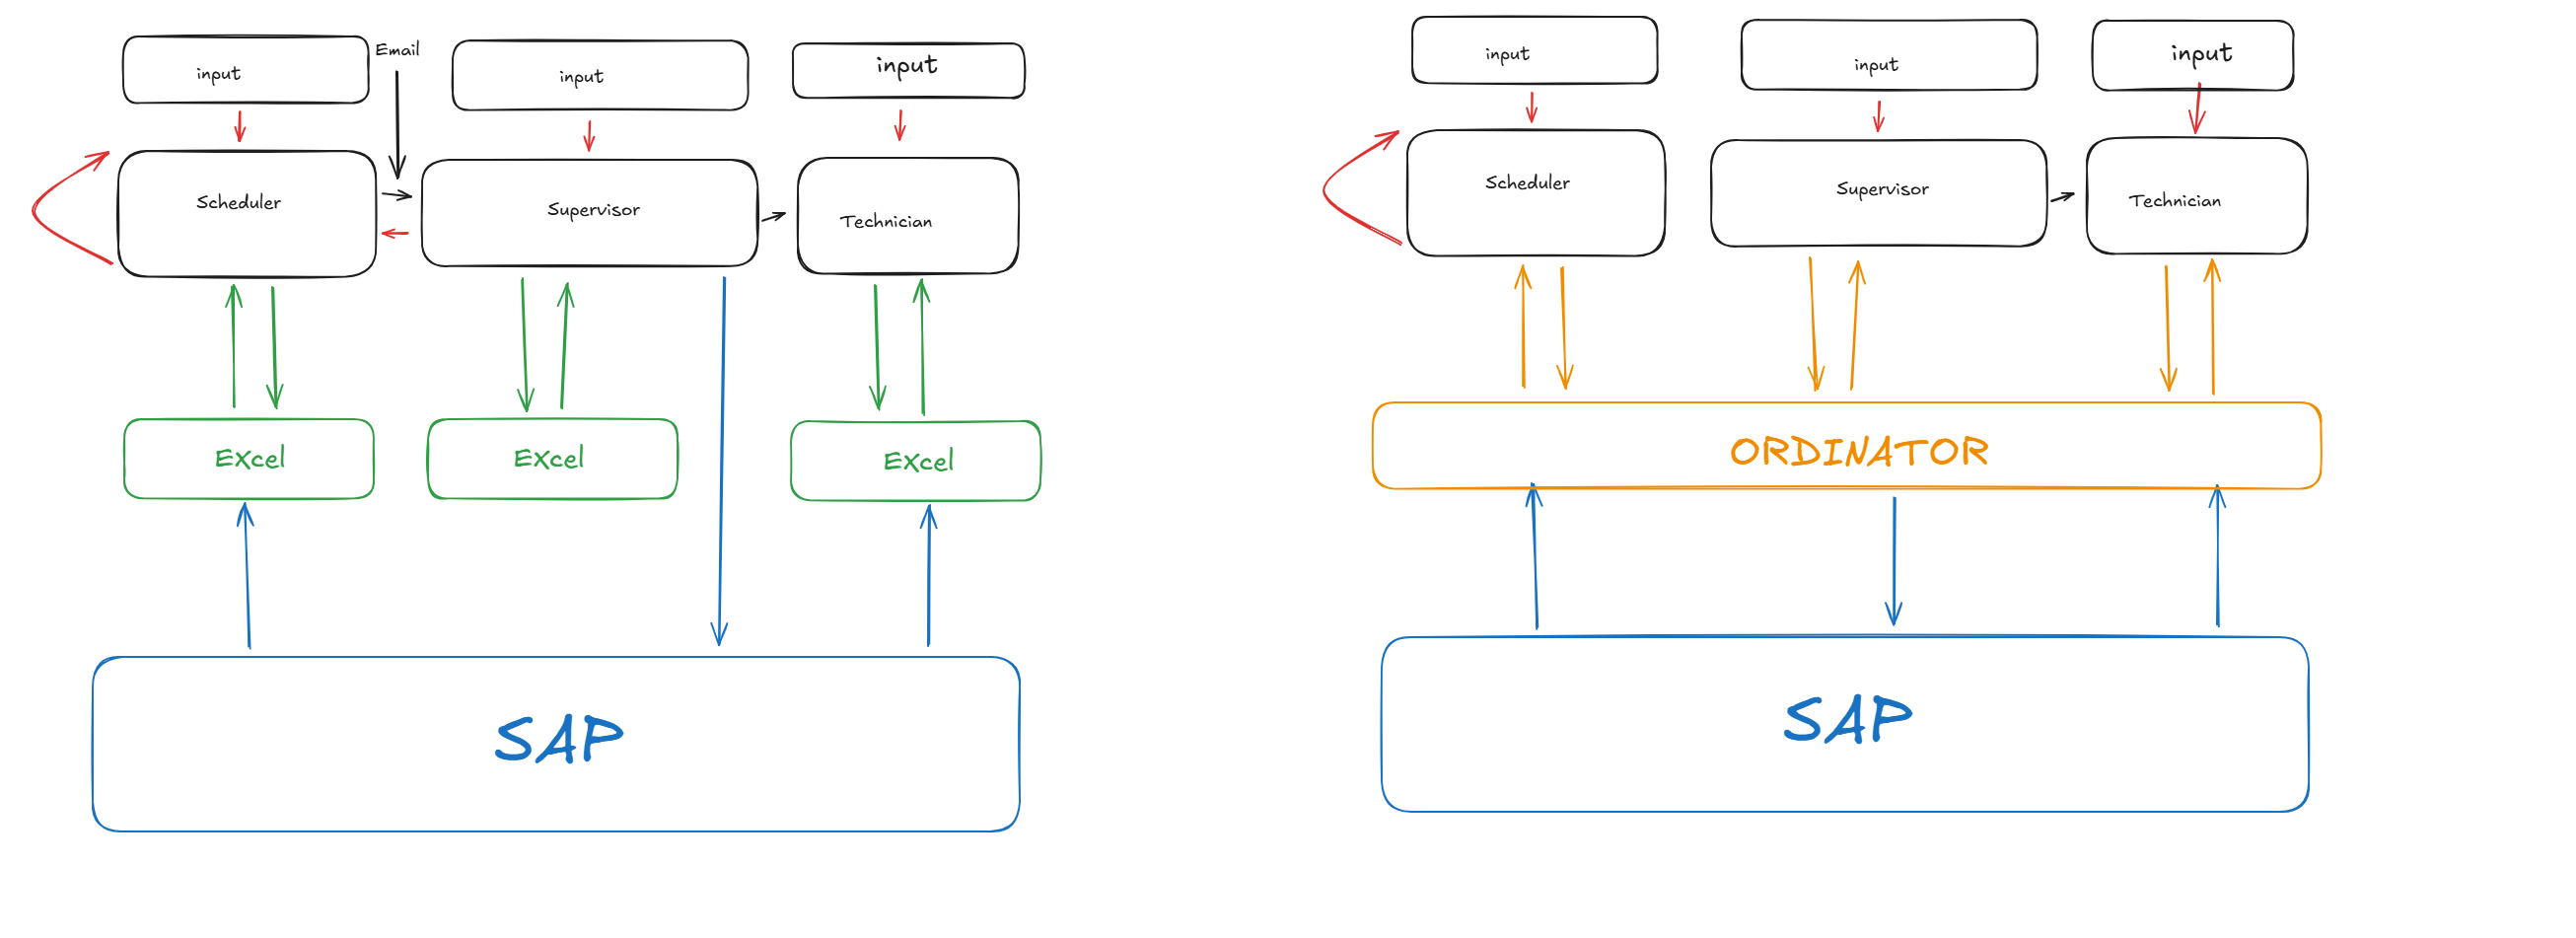
\includegraphics[width=1.0\textwidth]{project-plans/scipo-total/figures/scheduling-as-is-to-be.png}

\end{figure}
\begin{figure}
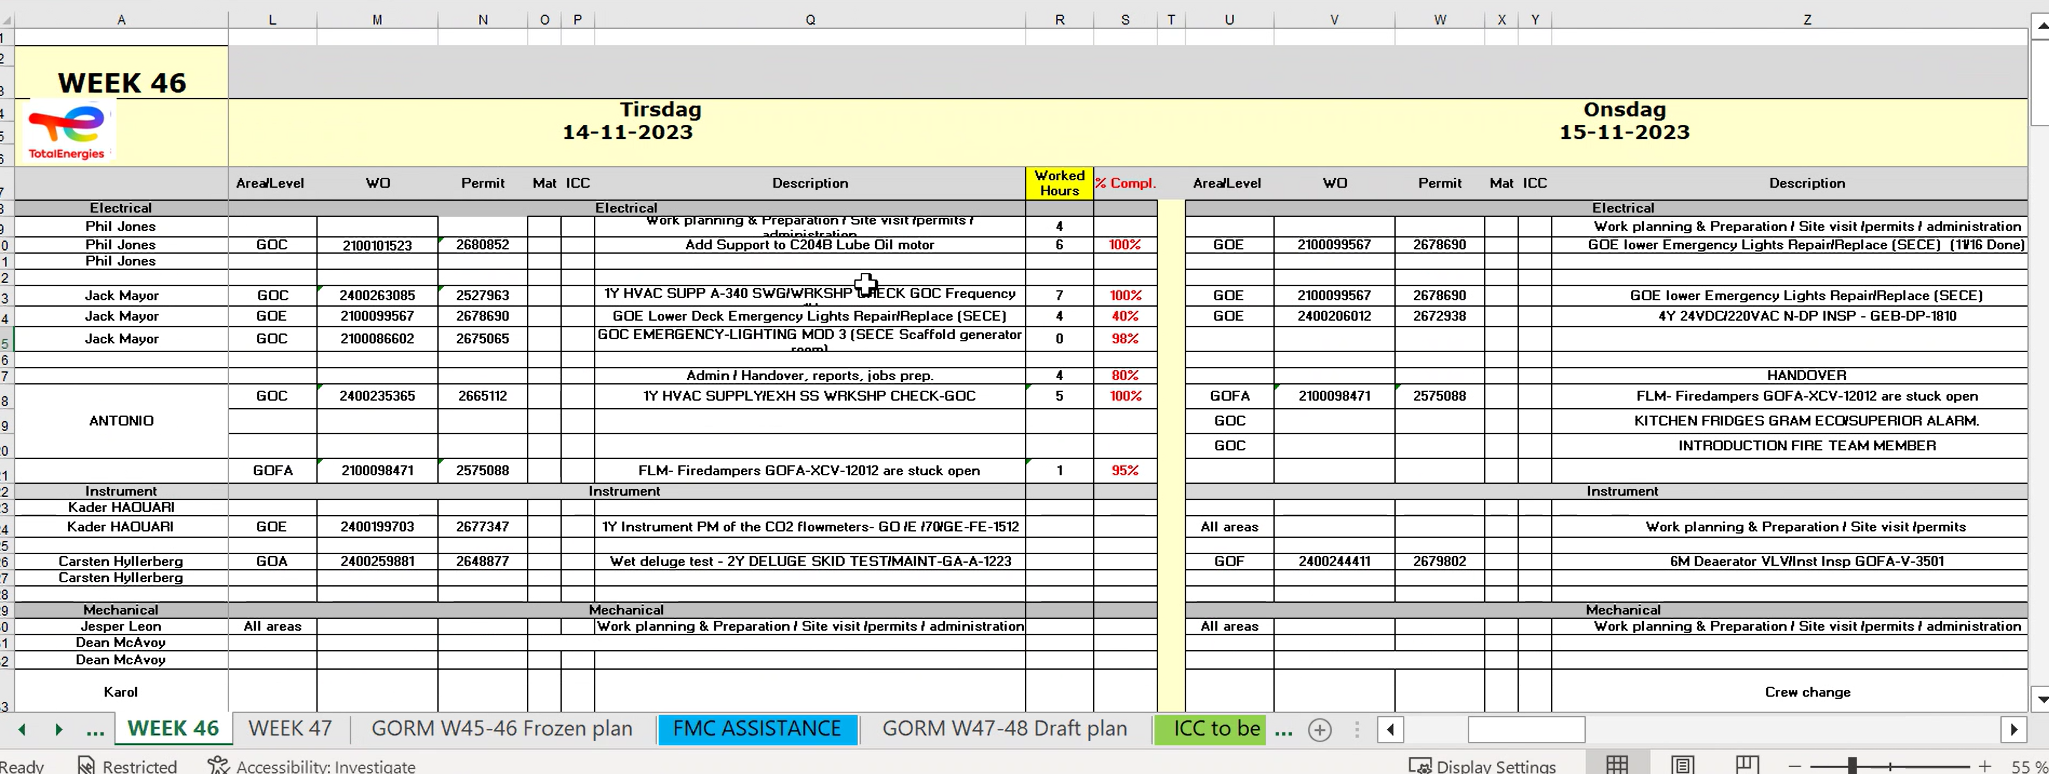
\includegraphics[width=1.0\textwidth]{project-plans/scipo-total/figures/technician-excel.png}
\end{figure}
\section{Envisioned Future}

What do we not know:
\begin{itemize}
    \item Supervisor is a big unknown. How do they work with the information? Do all supervisors do the same?
    \item Do they know what would be the best for them? DO we?
    \item What should be the main focus to get a minimum viable product?
    \item How mature the "engine" (ordinator) should be before trying to convince TotalEnergies?
\end{itemize}


\section{Company Structure}
Creating a company splitting the shares equally between the founders given Niels Henrik a share 10\%. 

\subsection{questions}
\begin{itemize}
    \item Should Total own anything?
    \item Does DTU need to own anything?
    \item Should there be a policy between risk taking and the amount of shares given to a person?
    \item Where should the company have headquarters?
\end{itemize}

\section{IP Concerns}
\begin{itemize}
    \item What rights do DTU have to software?
    \item Do we have a case where DTU are not willing to further this project alone and therefore we can do it ourselves without them?
    \item What does TotalEnergies expect? Do they expect this to be free or are they willing to fund this project even though it would be through a "subcontractor"?
\end{itemize}
\section{Convincing Total}
Does it make sense to pursue the idea?
How to make total commit themselves to spend hours on the project. What does this mean for who owns what?

Booking a meeting with the most relevant stakeholders, and getting a consensus on the project goals.

Drafting a budget, meaning how many hours there is needed to deliver certain milestones.

Working on an hourly basis, delivering weekly or monthly results.

What should the role of Christian's Ph.D. project be until we are ready to create the company?
One route (best-case-scenario): 
Christian takes leave of PhD in Autumn -> Total Energies hopefully is willing to pay for hours in development -> Christian and Sebastian works full time on paid project to develop -> Christian returns to finish PhD or project is so mature we cannot stop now.
\end{document}
